\documentclass{article}

\usepackage{amsmath, amsthm, amssymb, amsfonts}
\usepackage{thmtools}
\usepackage{graphicx}
\usepackage{setspace}
\usepackage{geometry}
\usepackage{float}
\usepackage{hyperref}
\usepackage[utf8]{inputenc}
\usepackage[english]{babel}
\usepackage{framed}
\usepackage[dvipsnames]{xcolor}
\usepackage{tcolorbox}
\usepackage{physics}
\DeclareMathOperator{\grd}{grad}
\colorlet{LightGray}{White!90!Periwinkle}
\colorlet{LightOrange}{Orange!15}
\colorlet{LightGreen}{Green!15}

\newcommand{\HRule}[1]{\rule{\linewidth}{#1}}

\declaretheoremstyle[name=Theorem,]{thmsty}
\declaretheorem[style=thmsty,numberwithin=section]{theorem}
\tcolorboxenvironment{theorem}{colback=LightGray}

\declaretheoremstyle[name=Proposition,]{prosty}
\declaretheorem[style=prosty,numberlike=theorem]{proposition}
\tcolorboxenvironment{proposition}{colback=LightOrange}

\declaretheoremstyle[name=Principle,]{prcpsty}
\declaretheorem[style=prcpsty,numberlike=theorem]{principle}
\tcolorboxenvironment{principle}{colback=LightGreen}

\setstretch{1.2}
\geometry{
    textheight=9in,
    textwidth=5.5in,
    top=1in,
    headheight=12pt,
    headsep=25pt,
    footskip=30pt
}

% ------------------------------------------------------------------------------

\begin{document}

% ------------------------------------------------------------------------------
% Cover Page and ToC
% ------------------------------------------------------------------------------
\section*{The Chain Rule}

\textbf{Example.} Let $f(x,y) = e^x \sin(xy)$. One can imagine
this describes the temperature of the plane at each point $(x,y)$.
Now imagine a bug moving in the plane with parametrization
$C(t) = (t^2, t^3)$. Then the temperature the bug is feeling at time $t$
is 
\[f(C(t))=e^{t^2}\sin(t^5).\]

Of course, we could compute the derivative of this directly,
but there's another way.

\textbf{Chain Rule.} Let $f$ be differentiable on an open set $U$
and let $C(t)$ be a differentiable curve contained in $U$. Then 
\[\frac{d}{dt} f\circ C(t) = (\grd f)(C(t)) \cdot C'(t).\] (Proof?
)

Suppose we're in the two-variable case and 
$C(t) = (x(t),y(t))$. We could rewrite the chain rule as
\[\frac{d}{dt} f\circ C(t) = \frac{\partial f}{\partial x} \frac{dx}{dt} + \frac{\partial f}{\partial y} \frac{dy}{dt}\]
where the partial derivatives are of course evaluated at $(x(t),y(t))$.


\textbf{Example.} Let $f(x,y,z) = x^2 y z$ and 
$C(t) = (x(t),y(t),z(t)) = (e^t, t, t^2)$.
Then 
\begin{align*}
(f\circ C)'(t) &= (D_1 f) x'(t) + (D_2 f) y'(t) + (D_3 f) z'(t)\\
&= 2xyz e^t + x^2 z  + x^2 y (2t)\\
&= 2e^{2t} t^3 + e^{2t} t^2 + 2e^{2t} t^2.
\end{align*}

There are situations where we need only use the standard single variable chain rule.
\textbf{Example.}
Let $f(x,y,z)=\sin(x^2-3yz+xz)$.
Then 
\[\frac{\partial f}{\partial x} = \cos(x^2-3yz+xz)(2x + z).\]
% ------------------------------------------------------------------------------
% ------------------------------------------------------------------------------

\section*{Tangent Plane}
Let $f(x,y,z)$ be a function on $\mathbb{R}^3$. Imagine that $f$ models the 
temperature at each point of the space and that we have
a bug moving along a curve $B(t) = (x(t),y(t),z(t))$ in space. 
Assume the bug started at a point with a comfortable temperature $k$
and so decides to stick to points with temperature $k$. That is,
the bug is moving on the level surface
\[f(x,y,z)=k.\]
That is, we have for all $t$ that
\[f(B(t))=k.\]
Applying chain rule, we have
\[(\grd f)(B(t))\cdot B'(t) = 0.\]
So the gradient of $f$ is perpendicular to the path of the bug
at every point.

In general, if we fix a point $P$ on a level surface $f(x,y,z)=k$ and look at all
differentiable curves passing through $P$ at, say, $t=0$, the above computation shows that all such curves
will be be perpendicular to $\grd{f}(P)$ at $t=0$ (see the following figure from Lang).
\begin{figure}[h]
    \centering
    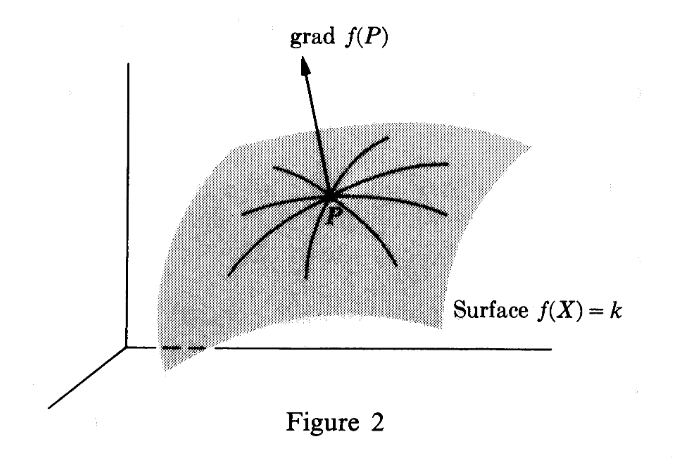
\includegraphics[scale = 0.5]{tangent1.PNG}
\end{figure}
Thus, in a very real sense, $\grd f(P)$ is perpendicular to the surface $f(x,y,z)=k$ itself.
This leads to the following definition.

\textbf{Definition.} The \textbf{tangent plane} to $f(X)=k$ at $P$ is the plane through $P$,
perpendicular to $\grd f(P)$.

\textbf{Example.} Find the tangent plane to $x^2+y^2+z^2=3$ at the point $(1,1,1)$. 

Note that this a level surface of the function $f(x,y,z)=x^2+y^2+z^3$ (corresponding to $f=3$). 
So our normal vector is $N = (2x,2y,2z)|_{(1,1,1)} = (2,2,2)$. The plane equation is then
\[(2,2,2)\cdot(x-1,y-1,z-1)=0,\]
or
\[x+y+z=3.\] 

We can use the same techniques to find tangent lines to curves in $\mathbb{R}^2$.

\textbf{Example.} Find the tangent line to $x^2y + y^3 = 10$ at $P=(1,2)$.

We set $f(x,y,)=x^2y+y^3$. Then $\grad(f)(P)=(4,13)$. Using the plane equation, our line is described by 
\[4x+13y=30.\]

If a surface is described as the graph of $z=g(x,y)$, we can still use the techniques above by noting
that the surface described by $z=g(x,y)$ is a level surface of the three-variable function $w(x,y,z,)=g(x,y)-z$.
In fact, one sees that the surface is precisely the level set corresponding to $w=0$. So a normal vector
to the surface is given by
 \[\grd w = \left(\frac{\partial g}{\partial x}, \frac{\partial g}{\partial y},-1\right).\]


 \section*{Directional Derivative}

We aim to investigate the rate of change of a function. 
Specifically, we're standing at some point $P$ in the domain of $f$
and start walking in the direction of a vector $A$ and want
to study the change in $f$. 

Let $P$ be a point and $A$ a \emph{unit} vector and look at the function
\[f(P+tA).\]
Chain rule gives us
\[\frac{d}{dt} f(P+tA) = \grd f (P+tA) \cdot A.\]
Evaluating at $t=0$, the right hand side is $\grd f(P) \cdot A$.
This leads to the definition of the directional derivative.

\textbf{Definition.} The \textbf{directional derivative} of $f$
at $P$ in the direction of $A$ is 
\[D_A f (P)= \grd f (P) \cdot A.\]

We note that for a function $z=f(x,y)$, this derivative can be 
interpreted geometrically as the slope of a tangent to the curve
formed by slicing the surface with the plane parallel to the $z$-axis
and the line $P+tA$.

\textbf{Example.} $f(x,y) = x^2 + y^3$, $B=(1,2)$. Find 
$D_B f (-1,3)$.

Note that $B$ is not a unit vector, so let's put 
$\hat{B} = \frac{1}{\sqrt{5}}(1,2)$. So really we're after $D_{\hat{B}} f (-1,3)$.
Plugging things in, have
\[D_{\hat{B}} f (-1,3) = (2x,3y^2)\bigg\vert_{(-1,3)} \cdot \left( \frac{1}{\sqrt{5}}(1,2) \right) = 52/\sqrt{5}. \]

If $P$ is a point and $A$ is a unit vector, we have
\[D_A f (P)= \grd f (P) \cdot A = \norm{\grd f(P)}\cos\theta,\]
where $\theta$ is the angle between $A$ and $\grd f(P)$ and $\norm{A}$
doesn't appear since it equals 1.

From this we get two interesting observations. One is that
the gradient points in the direction of steepest increase. The other
is that in this direction, the rate of change is $\grd f (P)$.
Similarly, $-\grd f(P)$ points in the direction of steepest decrease.

\end{document}